\section{Fourier Integral Method}
\begin{frame}{Fourier Integral Method}
  \begin{itemize}
  	\item The density spectrum $s(\omega)$ created in the last sections can be used directly to generate unconditional realizations. This is the \textit{Fourier Integral Method (FIM)} \cite{pardo1993fourier}.
    \item The covariance table $C(h)$ can be generated using the following equation:
    $$
    C(h) = z * z = \mathscr{F}^{-1}[Z(\omega) \cdot Z(\omega)],
    $$
    
    $$
    s(\omega) = Z(\omega) \cdot Z(\omega),
    $$
    where $z(p)$ is data function in the point $p=(x,y,z)$, $*$ is the convolution operation and $Z(\omega) = \mathscr{F}[z(p)]$,
    \item Remembering that $Z(\omega)$ can be written as $Z(\omega)=|Z(\omega)|e^{i\theta}$. And if a function $f(y)$ is real, the angle $\theta$ is 0 for all $y$. 
    \item Then, the density spectrum $s(\omega)$ is given by $s(\omega) = |Z(\omega)|^2$.
  \end{itemize}
\end{frame}

\begin{frame}{Fourier Integral Method}
  \begin{itemize}
  	\item The density spectrum $s(\omega)$ can be used  to recover the magnitude of the original data function $z(p)$, because $|Z(\omega)| = \sqrt{s(\omega)}$. Remembering that $s(\omega) \geq 0$ is a positive function. Also, $\sum |s(\omega)| = C(0)$.
    \item In the FIM simulation, the lost angle $\theta(\omega)$ is re-added to the density spectrum  $\sqrt{s(\omega)}$. And data conditioning is realized using error kriging.
    \item The unconditional simulation is done generating random angles $\theta(\omega)$ from an uniform distribution $U(-\pi,\pi)$.
    \item Then, the unconditional realization $z^{r}(p)$ is generated using the equation $z^{r}(p) = \mathscr{F}^{-1}[\sqrt{s(\omega)}e^{i\theta(\omega)}]$. Without loss of generality, let assume that $Z^{r}(p)=\sqrt{s(\omega)}e^{i\theta(\omega)}$ is even (this assure that the inverse is a real function).
  \end{itemize}
\end{frame}

\begin{frame}{Unconditional simulation using Covariance table and FIM}
\begin{figure}[!ht]
  \caption{Example of unconditional simulation using a smoothed covariance table generated using the Walker Lake dataset.}
  \centering
    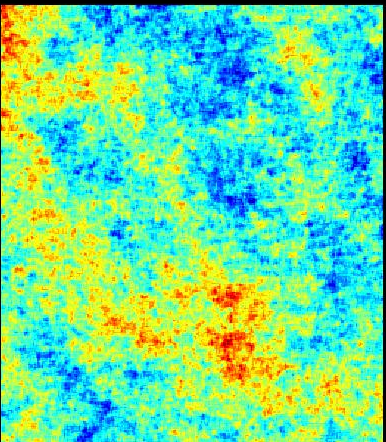
\includegraphics[height=0.5\textheight]{figs/sim_cov_table.png}
    \label{cov_table_sim.fig}
\end{figure}
\end{frame}


\begin{frame}{Advantages of Fourier Integral Method}
\begin{itemize}
	\item FIM doesn't need a random path.
    \item The generated covariance table from data can be used directly to generate the unconditional simulations and conditioning.
    \item FIM is embarrassingly parallel.
\end{itemize}
\end{frame}

\begin{frame}{Drawbacks of Fourier Integral Method}
\begin{itemize}
	\item It's highly dependent on the correct adjust of the simulation grid. The grid discretization (cell size) is directly related to the quality of simulation. A more continuous spatial input data demands a small cell size. This fact is explained by the Nyquist Sampling Theorem \cite{pardo1993fourier}. 
    \item The FFT in non-equally sampled vector of data isn't a trivial problem \cite{keiner2009using}.
\end{itemize}
\end{frame}




